%%
%% This is file `lexample.tex',
%% Sample file for siam macros for use with LaTeX 2e
%%
%% October 1, 1995
%%
%% Version 1.0
%%
%% You are not allowed to change this file.
%%
%% You are allowed to distribute this file under the condition that
%% it is distributed together with all of the files in the siam macro
%% distribution. These are:
%%
%%  siamltex.cls (main LaTeX macro file for SIAM)
%%  siamltex.sty (includes siamltex.cls for compatibility mode)
%%  siam10.clo   (size option for 10pt papers)
%%  subeqn.clo   (allows equation numbners with lettered subelements)
%%  siam.bst     (bibliographic style file for BibTeX)
%%  docultex.tex (documentation file)
%%  lexample.tex (this file)
%%
%% If you receive only some of these files from someone, complain!
%%
%% You are NOT ALLOWED to distribute this file alone. You are NOT
%% ALLOWED to take money for the distribution or use of either this
%% file or a changed version, except for a nominal charge for copying
%% etc.
%% \CharacterTable
%%  {Upper-case    \A\B\C\D\E\F\G\H\I\J\K\L\M\N\O\P\Q\R\S\T\U\V\W\X\Y\Z
%%   Lower-case    \a\b\c\d\e\f\g\h\i\j\k\l\m\n\o\p\q\r\s\t\u\v\w\x\y\z
%%   Digits        \0\1\2\3\4\5\6\7\8\9
%%   Exclamation   \!     Double quote  \"     Hash (number) \#
%%   Dollar        \$     Percent       \%     Ampersand     \&
%%   Acute accent  \'     Left paren    \(     Right paren   \)
%%   Asterisk      \*     Plus          \+     Comma         \,
%%   Minus         \-     Point         \.     Solidus       \/
%%   Colon         \:     Semicolon     \;     Less than     \<
%%   Equals        \=     Greater than  \>     Question mark \?
%%   Commercial at \@     Left bracket  \[     Backslash     \\
%%   Right bracket \]     Circumflex    \^     Underscore    \_
%%   Grave accent  \`     Left brace    \{     Vertical bar  \|
%%   Right brace   \}     Tilde         \~}


\documentclass[final]{siamltex}

% definitions used by included articles, reproduced here for
% educational benefit, and to minimize alterations needed to be made
% in developing this sample file.

\newcommand{\pe}{\psi}
\def\d{\delta}
\def\ds{\displaystyle}
\def\e{{\epsilon}}
\def\eb{\bar{\eta}}
\def\enorm#1{\|#1\|_2}
\def\Fp{F^\prime}
\def\fishpack{{FISHPACK}}
\def\fortran{{FORTRAN}}
\def\gmres{{GMRES}}
\def\gmresm{{\rm GMRES($m$)}}
\def\Kc{{\cal K}}
\def\norm#1{\|#1\|}
\def\wb{{\bar w}}
\def\zb{{\bar z}}

% some definitions of bold math italics to make typing easier.
% They are used in the corollary.

\def\bfE{\mbox{\boldmath$E$}}
\def\bfG{\mbox{\boldmath$G$}}


%%%%%%%%%%%%%%%%%%%%%%%%%%%%%%%%%%%%%%
% Actual stuff starts here


%% encoding
\usepackage[utf8]{inputenc}
\usepackage[english]{babel}

%% bibtex
\usepackage[comma,authoryear]{natbib}
%% Math packages
\usepackage{amsmath}
\usepackage{amsfonts}
\usepackage{amssymb}
\usepackage{mathrsfs}

\usepackage{color}
\usepackage{hyperref}
\usepackage{graphicx}
\usepackage{listings}

\newcommand{\mycomment}[1]{{\color{blue} #1}}

\title{Probabilistic Program Induction for Model-Based Reinforcement Learning}

% The thanks line in the title should be filled in if there is
% any support acknowledgement for the overall work to be included
% This \thanks is also used for the received by date info, but
% authors are not expected to provide this.

\author{Zenna Tavares and Max Siegel\thanks{Department of Brain \& Cognitive Sciences, Massachusetts Institute of Technology}
}
\begin{document}

\maketitle

\begin{abstract}
Model-based reinforcement learning (RL) is a powerful method for acting in unknown environments, but most approaches require specific, limiting assumptions about the world model.
Probabilistic program induction promises flexible, universal learning from data.
We present an outline of a method for inducing and using adaptive generative models in reinforcement learning. 
The approach is to learn probabilistic programs from experience and choose actions by sparse sampling.
We describe several systems that we have built towards this goal. 
RL-Church is a system based on the Church programming language that allows for easy specification of complex generative models in RL tasks.
Stochastic Javascript is a extension of Javascript which allows for fast computation and easy Internet data collection. These tools aid development of improved RL agents.
\end{abstract}

\begin{keywords}
Probabilistic program induction, model-based reinforcement learning, Church, Stochastic Javascript
\end{keywords}

\section{Introduction}
Reinforcement learning (RL) is a successful field of machine learning that has enjoyed much practical application, and is often the method of choice when acting in unknown or partially-unknown environments.
However, there are simple examples of problems that humans solve effortlessly but pose challenges for standard RL algorithms. 
Consider the finite-state automaton in Figure 1 (drawn from \citet{dearden}).\begin{figure}
\begin{center}

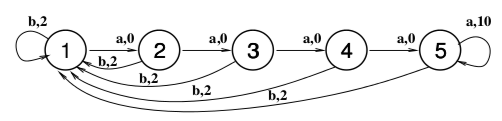
\includegraphics[scale=.4]{chain}

\end{center}
\caption{The chain problem; with probability .2, each action \emph{a} or \emph{b} results in a transition to the starting state 1. State 5 gives much greater reward than state 1, but standard RL algorithms fail to discover it.}
\end{figure}
The task is difficult because before the agent reaches the fifth stage, all of the evidence received suggests that the best strategy is to remain at the first state.
Yet it seems clear that the potential rewards are sufficient to warrant visiting each state.
This is an example of the \emph{exploration-exploitation tradeoff} \citep{wolpert}: to maximize final reward, when should one decide to quit roaming and settle down?

Recent work \citep{shawn} has shown that humans perform very well on the chain problem, finding the best state hundreds or thousands of times faster than most RL algorithms.

What could account for such dramatic differences?
Humans seem to perform very well on problems with clear structure, possessing a strong inductive bias towards simplicity.
Conversely, human performance is very poor in arbitrarily general RL environments \citep{finale}. 

To capture this apparent feature of human learning, we used techniques from Bayesian RL and probabilistic program induction to create a principled, (semi-) tractable method for learning to act in unknown environments. 
Church \citep{church} is a probabilistic programming language that allows for flexible, compositional representation of generative models. 
Since its release, there has been steadily increasing interest in Bayesian program induction using Church \citep{hwang}.
This work uses a program length prior to learn concise models from data.
This framework seems well suited to the problem at hand; the length prior prefers structured models that abstract over states and actions, without specifying their precise form.

Both probabilistic programming and Bayesian RL pose significant computational difficulties. Bayesian RL requires that one maintain a posterior distribution over possible world models, which we represent using Church programs. 
Exact action selection in Bayesian RL requires exact planning, which is impossible for infinite horizon problems and intractable for finite horizon problems \citep{puterman}.
We use sparse sampling for action selection, which maintains our Bayesian approach while making planning tractable \citep{kearns}.
Finally, probabilistic program induction is perhaps the most difficult computational task that we face; calculating the posterior probability of programs is intractable \citep{vikash}. 
We use two strategies to enable computation.
Rather than attempt to model the posterior probability directly, we draw (approximate) samples from the posterior distribution; this is a ubiquitous strategy in machine learning and computational statistics \citep{mackay}. 
To find high-probability programs, we use heuristics that favor abstraction (drawn from \citet{hwang}).

The plan of the paper is as follows. 
In Section 2, we review background material. 
In Section 3, we outline our proposed method. 
In Section 4, we describe RL-Church, a RL system based on the Church programming language. 
In Section 5, we describe Stochastic Javascript, an extension of the Javascript programming language.
To conclude, we discuss possible applications and future research directions.
\section{Background}
\subsection*{Reinforcement Learning}
Reinforcement learning (RL) is a formalization of the problem of learning to behave optimally in unknown environments \citep{suttonbarto}. An environment is a tuple $(S,A,T,R)$, where $S$ is a set of \emph{states}, $A$ is a set of (possibly state-dependent) \emph{actions}, $T: S\times A \to S$ is a stochastic state \emph{transition function}, and $R: S\times A -> \mathbb{R}$ is the \emph{reward} of taking action $a$ in state $s$.

The classical theory of RL typically solves the problem by estimating $(R,T,A)$ and using techniques from the theory of MDPs (see below). This effectively disregards the exploration aspect of the tradeoff mentioned above . Other techniques try to estimate and incorporate the \emph{value of perfect information} and other heuristics to encourage exploration.
\subsection*{Markov Decision Processes}
Markov Decision Processes (MDPs) \citep{puterman} are a subset of RL problems; they assume that the state, action, transition function, and reward functions are known. Thus the problem reduces to calculating the optimal way to act. For small MDPs, this is straightforward; algorithms for exact calculation have been known since the 1950s. For large MDPs,  approximate techniques are required. Sparse sampling is one such method.\newpage
\subsection*{Sparse Sampling}
Sparse sampling \citep{kearns} is a method for choosing actions to maximize rewards in MDPs for which the learning agent has a generative model of the world. 
A \emph{generative model} is a probability distribution $p: S\times A \to S\times \mathbb{R}$ that, given a state and action, returns a new state and a reward. 
Sparse sampling techniques sample from this model to grow a state-action-reward tree to a specified depth, then transform this tree into an approximate MDP and use standard methods to solve it. 
The following listing shows our implementation of sparse sampling in Church.

\lstset{language=Lisp}
\begin{lstlisting}[caption={Sparse Sampling},label=sparse]
; Kearns et al. Sparse sampling algorihtm
(define sparse-sampling
  (lambda (depth num-samples discount model state 
                 possible-actions state-queries)
    (let
        ((q-star (estimate-q depth num-samples discount
                             model state possible-actions
                             state-queries)))
      (list-ref possible-actions (argmax (lambda (x) x) q-star)))))


; Estimate value
(define estimate-v
  (lambda (depth num-samples discount model state
                 possible-actions state-queries)
    (let 
        ((q-star (estimate-q depth num-samples discount
                             model state possible-actions
                             state-queries)))
      (max-in-list q-star))))

; For each action in possible actions generate C samples
; And compute the reward until max depth
(define estimate-q
  (lambda (depth num-samples discount model state
                 possible-actions state-queries)
    (cond ((zero? depth)
           (list 0))
          (else
           (map (lambda (action)
                  (/ (sum-rewards num-samples
                                  num-samples depth
                                  discount model
                                  state action
                                  possible-actions
                                  state-queries)
                     num-samples))
                possible-actions)))))

; Recursive function to applied to evevery action
(define sum-rewards
  (lambda (sample-num num-samples depth
                      discount model state action
                      possible-actions state-queries)
    (if (zero? sample-num)
        0
        (let ((state-reward (model state action state-queries)))
          (+
           (cdr state-reward)
           (* discount (estimate-v (- depth 1)
                                   num-samples
                                   discount
                                   model state
                                   possible-actions
                                   state-queries))
           (sum-rewards (- sample-num 1) num-samples
                        depth discount
                        model state action
                        possible-actions state-queries))))))
\end{lstlisting}

\subsection*{Probabilistic Program Induction}
Probabilistic program induction techniques attempt to learn programs from data. 
We shall focus on \emph{Bayesian} program induction, which assumes a prior probability distribution $p(M)$ over programs. 
Using Bayes' theorem, $p(M|D)\propto p(D|M)p(M)$, these techniques estimate the posterior probability distribution over programs \citep{hwang}.
\subsection*{Church}
Church \citep{church} is an extension of the programming language Scheme \citep{steele-sussman78} to allow stochastic functions.
It allows flexible specification of generative models (it can express any computable probability distribution), and supports general-purpose probabilistic inference.
A flurry of recent work (see the Church Wiki) has focused on probabilistic program induction using Church.

\section{Model-Based Reinforcement Learning by Probabilistic Program Induction}
To encourage generalization and abstraction for model-based RL, we propose to induce Church programs as models of the world. 
Following \citep{hwang}, we choose a program length prior $p(M)\propto \exp(-\alpha |M|)$ and estimate the likelihood $p(D|M)$ by a combination of brute-force frequency estimation of and analytic evaluation given the model. 
Samples are drawn from the posterior $p(M|D)\propto p(D|M) p(M)$ using Markov Chain Monte Carlo, using search moves that favor abstraction and deargumentation.
For each step taken by the RL agent, we draw a number of program samples $p$ from $p(M|D$, and draw state-action-reward sample trajectories from the generative model specified by each program.

Sparse sampling is used to calculate the posterior distribution over actions (combining the sample trajectories from all  sampled programs), which we sample from to specify the agent's decision. 
The early stages of exploration will be essentially random;  as it collects more data, we expect the agent to both make better predictions of transition and reward probabilities and to better predict the properties of as yet unobserved states.

We view our proposal as having two main advantages. First, it is in some sense fully Bayesian. Rather than make point estimates at any step, we sample directly from the posterior distribution over the quantities of interest. Second, although it is most likely computationally intractable for any but the simplest RL problems, it provides a framework for exploring further approximations to optimal Bayesian RL.
To facilitate such exploration, we have developed several tools for probabilistic programming and reinforcement learning.

\section{Stochastic Javascript}
To meet the resource requirements of both reinforcement learning and program induction we developed a stochastic extension of the JavaScript programming language.
JavaScript is a dynamic and weakly typed multi-paradigm language, with C-like syntax \citep{javascript}.
In spite of its name, it bears little semantic resemblance to Java and instead derives many of its ideas from Scheme, with support for first class functions, closures, lambda expressions and an $eval$ procedure to evaluate dynamically generated code.
It also offers many of the features associated with more commonly used imperative languages, such as a prototypical object model, the modification of state, and the ability to introduce side-effects in functions.

Competition between browser vendors has in recent years taken place on the performance front, leading to a tremendous increase in the speed of JavaScript implementations, which now routinely outperform other interpreted languages in benchmark tests.
A large contribution to this progress stems from the adoption of just-in-time compilation (JIT) techniques, which sits somewhere in between interpretation and static (ahead-of-time) compilation \citep{Aycock03}.
This combination of language and implementation properties make JavaScript particularly attractive for this program induction, since inducted programs will be compiled to native code on the fly.

\subsection*{Implementation}
Stochastic JavaScript implements three properties of Church: elementary random primitives (ERPs), stochastic operators and implementations of \verb+QUERY+.

The following listing  demonstrates the implementation of an Elementary Random Primitive of a discrete Poisson distribution and is equivalent to the \verb+(poisson lambda)+ function found in Church.

\lstset{language=C}
\begin{lstlisting}[caption={ERP of Poisson Distribution},label=poisson]
var poissionRnd = function (lambda) {
        var L = Math.exp(-lambda);
        var k = 0;
        var p = 1;
        do {
            k = k + 1;
            p = p * Math.random();
        }
        while (p > L);
        return k - 1;
    }
\end{lstlisting}

\ref{fig:sif} is a implementation of a stochastic \verb+if+ operator, which will take the wrong path with some probability, this may contribute to softening the space of possible programs.

\lstset{language=C}
\begin{lstlisting}[caption={Stochastic If Operator},label=sif]
vvar sIf = function(noiseLevel, predicate,
                             consequent, alternate) {
    noisyPredicate = flip(noiseLevel) ? predicate: !predicate;
    if (noisyPredicate) {
        return consequent;
    } else {
        return alternate;
    }
}
\end{lstlisting}

\subsection*{Conditional Inference}
To support conditional inference Church generalises evaluation to \textit{conditional simulation} \citep{church} of any generative process, organising computation around a procedure \verb+(QUERY <expression> <environment> <predicate>)+.
\verb+QUERY+ simulates from the distribution of values of a given expression given that the predicate is true.
As in Church, we first provide an implementation of \verb+QUERY+  in \cite{querydad}, which takes as arguments an expression and predicate and returns a sample from the conditional distribution on values induced by the expression.
We use here rejection sampling, which equates to recursively simulating the underlying process and accepting only if the predicate evaluates as true.
Listing \ref{fig:m}  extends this to a lexicalised version of \verb+query+, which for purposes of convenience provides a method to name random variables, shared across all evaluations; in effect constructing the elements of a random world.
One further difference between our implementation of \verb+query+ and \verb+lex-query+ is the representation of an expression as a function instead of as a string as required for \verb+eval+.
Functions can be dynamically created with \verb+new Function("code as string")+, which parses the code stored in a string into a function object, which can then be called.
These functions cannot affect local variables because the code runs in a separate scope and hence, the JIT compiler is able to make assurances about the function and infer better optimisations.

\lstset{language=C}
\begin{lstlisting}[caption={A Rejection Sampling Implementation of Query},label=query]
var query = function (expression, predicate) {
        var val = eval(expression);
        if (predicate(val) === true) {
            return val;
        } else {
            return query(expression, predicate);
        }
    }
\end{lstlisting}

\lstset{language=C}
\begin{lstlisting}[caption={Lexicalised sampling based query},label=query]
var lexQuery = function (lexicons, expression, predicate) {
        var evaluatedLexicons = [];
        for (var i = 0; i < lexicons.length; ++i) {
            evaluatedLexicons[i] = lexicons[i]();
        }
        var val = expression.apply(this, evaluatedLexicons);
        if (predicate.apply(this, val) === true) {
            return val;
        } else {
            return lexQuery(lexicons, expression, predicate);
        }
    }
\end{lstlisting}

Rejection sampling is expected to intractable in general, so here we outline an approximation of query following the method outlined in (WINGATE LIGHTWEIGHT PAPER).
The general idea is to give each ERP of a probabilistic program a unique name representing its position in the stack-trace, and then converting these stochastic functions into deterministic ones, effectively forcing a particular trace through the program.
We can then implement a Markov Chain through the space of program traces by modifying the values of these ERPs according to the Metropolis Hastings algorithm.
The inherent statefulness of this procedure is ill suited to a functional language, but as stated previously JavaScript permits the modificatio of global state.
To realise this we maintain a database to which ERP sampled values are saved to, or retrieved from in a manner outlined in detail in (WINGATE), and compute the likelihood of the all random choices made during a program ER $x$ by 

\begin{equation}
p(x) = \prod_{k=1}^K p_{t_k}(x_k \vert \theta_{t_k},x_1,...,x{k-1})
\end{equation}

where $k$ is the $k^{th}$ encountered ERP and $\theta$ are parameters of the distribution.
In order for each ERP to control the values of ERPs to be either sampled or retrieved from the database, we modify their (for example see (MODIFIED POISSON) to take in a $(database, logLikelihood$ pair as arguments in addition to any parameters.
Currently this modification has happened manually, but automatic code translation of ERPs is certainly feasible.

\lstset{language=C}
\begin{lstlisting}[caption={Modified Poission ERP for MCMC},label=modERP]
var poissionRnd = function(database, logLikelihood, lambda) {
    var currentParams = {
        type: 'poissionRnd',
        theta: arguments
    };

    var name = generateNameFromStackTrace();
    if (name in database 
            && currentParams.type == dbParams.type) {
        dbParmas = database[name];
        if (currentParams.theta == dbParams.theta) {
            logLikelihood = logLikelihood +
                                     dbParams.logLikelihood
        } else {
            var l = Math.log(computeLikelihood());
            database.name.l = l;
            logLikelihood = logLikelihood + l;
        }
    } else {}

    var L = Math.exp( - lambda);
    var k = 0;
    var p = 1;
    do {
        k = k + 1;
        p = p * Math.random();
    }
    while (p > L);
    return k - 1;
}
\end{lstlisting}

\section*{Implementation details of RL-Church}
RL-Church is designed to be agnostic to the domain of the problem.
The main algorithm, demonstrated in the following code takes as input a state, a list of possible actions, and \verb+state-queries+ list of possible queries to that state.
Our important detail is the layer of abstraction afforded with the use of \verb+state-queries+.
Although all observable state structure is contained within the \verb+state+ structure, all probing of the world must operate through the functions within \verb+state-queries+.
This allows us to modify our representation of the world, without having to modify our main learning algorithms.
It is also this set of functions, which are used in program induction to interrogate the state and learn regularities.

\begin{lstlisting}[caption={Main RL-Church Algorithm},label=rlmain]
(define do-learning
  (lambda (current-time state possible-actions state-queries)
    (cond
      (((list-ref state-queries 0) current-time state)
       (let* ((current-model (select-model 1.0 state-queries))
              (num-samples 3)
              (depth 3)
              (discount .7)
              (best-action (sparse-sampling
                            depth num-samples
                            discount current-model
                            state possible-actions
                            state-queries)))
         (begin
           (display current-time)
           (display "\n")
           (display best-action)
           ((do-learning (+ 1 current-time) state
                         possible-actions
                         state-queries)))))
       (else
        (display "Game over")))))
\end{lstlisting}

The algorithm is executed by creating an initial state, and suitable list \verb+state-queries+.

\section{Conclusion}
We have presented a proposal for a model-based reinforcement learning algorithm that employs probabilistic program induction to represent and induce flexible generative models.
In addition, we have developed two tools for research along this lines. RL-Church is an implementation of reinforcement learning in the Church programming language. Stochastic Javascript is a probabilistic programming language suitable for fast computation and Internet data collection. 


\bibliographystyle{siam}
\bibliography{induct}

\end{document}
